\documentclass[a4paper,11pt]{article}
\usepackage[utf8]{inputenc}
\usepackage{amsmath}
\usepackage{amsfonts}
\usepackage{amssymb}
\usepackage{graphicx}
\usepackage{braket}

\numberwithin{equation}{section}
\renewcommand\thesubsection{\alph{subsection}}
\newcommand{\bvp}[1]{\mathbf{#1}'}
\newcommand{\bv}[1]{\mathbf{#1}}


%opening
\title{Quantum II HW7}
\author{Vincent Baker}

\begin{document}

\maketitle

\section{Problem 1}
We consider the ground state of $^{61}_{28}Ni$ as a filled $3d^{10}$ level that has two electron holes.
We examine the energy level splitting due to spin alignment, electrostatic effects and spin-orbit coupling.\\

The energy level is first split into two separated levels by the spin-spin alignment. 
With two spin $\frac{1}{2}$ holes the total spin S can be 0 or 1.
The states with the spins aligned will have lower energy.\\
The spin levels are further split by the electrostatic hole-hole repuslion. 
The hole-hole repulsion is the same as electron-electron repulsion.
With two d holes ($\ell=2$) the total orbital angular momentum L can take on values from 0 to 4.
Higher L values will maintain a greater hole-hole separation and thus have a lower energy.\\
The states are further split by spin-orbit coupling. 
The sign of the spin-orbit coupling term in the Hamiltonian will be reversed since the holes have positive charge, flipping the direction of the orbital angular momentum.
This leads to states with greater total angular momentum J having lower energy.
\\
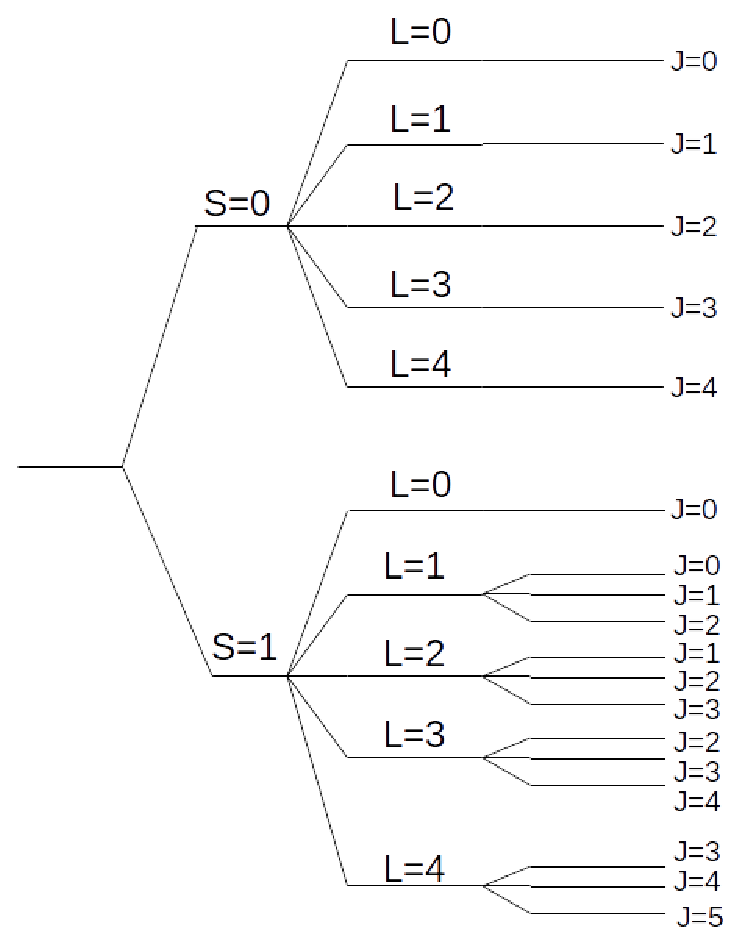
\includegraphics{LSsplitting}
\\
Both holes have quantum number n=3, and so in states with $\ell_1=\ell_2, s_1=s_2$ they would be identical particles. 
These energy levels are therefore forbidden by the Pauli exclusion principle. 
The forbidden states are $\ket{S=1,L=4}$, and $\ket{S=1,L=0}$ as the highest and lowest L states have both orbital and spin angular momentum the same.
\end{document}
